\section{Бутстреп оценки ошибки предсказания}
\subsection{Обзор}
В следующих двух разделах мы посомтрим, как можно использовать бутстреп для оценки ошибки предсказания. Для точной формулировки потребуются некоторые обозначения. Прежде чем перейти к ним обсудим основные идеи. Простейший бутстреп подход заключается в следующем: генерируется B бутстреп выборок для каждой из которых оценивается модель, затем каждая из моделей применяется к \textit{исходной выборке} и оценивается ошибка предсказания, таким образом, получаем B оценок ошибки предсказания. Общая оценка ошибки предсказания --- это среднее значение этих B оценок. В качестве примера в левом столбце таблицы 17.1 приведены десять оценок ошибок предсказания (<<err>>) для десяти бутстреп выборок для данных о гормонах, которые были описаны в разделе 17.2. Их среднее значение равно $2.52$, для сравнения, среднее значение для $\text{RSE} / n$ равно $2.20$.
\begin{figure}[H]
\center{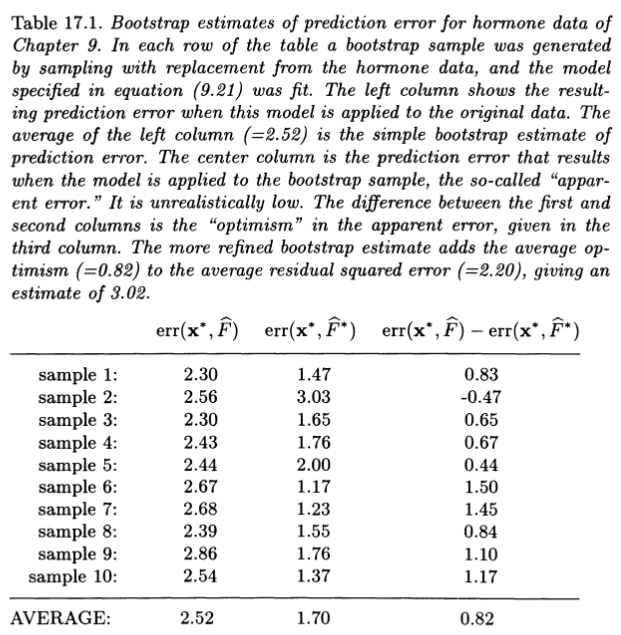
\includegraphics[width=1 \linewidth]{17/t17.6.1.1.png}}
\end{figure}

Такой простой бутстреп подход не очень хорош, но его легко можно улучшить. Посмотрим на второй столбец таблицы 17.1 он отображает ошибку предсказания для модели которая применяется к той же бутстрпеп выборки на которой и была обучена. Неудивительно, что значения во втором столбце в среднем ниже, чем в первом. Улучшенная бутстреп оценка основана на разнице между первым и вторым столбцом. Она называется <<оптимизм>> --- это величина, на которую средняя остаточная ошибка (или <<частота явных ошибок>>) занижает истинную ошибку предсказания. Общая оценка <<оптимизма>> --- это среднее значение B разностей между первым и вторым столбцом, в этом примере это значение равно $0.82$.


После того как <<оптимизм>> оценка получена, она складывается с явной частотой ошибок, так и получается улучшенная оценка ошибки предсказания. Здесь $2.20 + 0.82 = 3.02$. Конечно, $10$ бутстреп выборок --- это слишком мало. Если использовать $200$ бутстреп выборок, то бутстреп оценка будет равна $2.77$, а (optimism)??? оценка $0.80$, тогда улучшенная оценка ошибки прогноза будет равна $2.20 + 0.80 = 3.00$. По сути, тут происходит коррекция смещения явной частоты ошибок подобно тому, как мы сделали это в 10 главе.


\subsection{Некоторые детали}
Улучшение простого бутстреп подхода происходит посредством устранения разницы между строками таблицы 17.1, что во многом аналогично устранению (block effects)??? в двухфакторном дисперсионном анализе. Чтобы лучше понять обоснование бутстреп процедуры, нам нужно мыслить в терминах вероятностных моделей.

В седьмой и девятой главах мы описываем два бутстреп метода регрессионных моделей. Второй метод, на котором мы остановимся, обрабатывает данные $\textbf{x}_{i} = (\textbf{c}_{i}, y_{i}), i = 1, 2,\ldots,n$ как независимые и одинаково распределенные из многомерного распределения $\text{F}$. Напомним, что $\textbf{c}_{i}$ может быть вектором, в данных по гормону $\textbf{c}_{i}$ --- это номер партии и время ношения $i$-го устройства. Назовем всю выборку $\textbf{x}$. Таким же образом можно сформулировать проблему классификации с помощью $y_{i}$, указывющему на класс, которому принадлежит $i$-ое наблюдение. Обсуждение, которое мы приведем далее, носит довольно общий характер и охватывает проблемы как регрессии, так и классификации.

Предположим, мы оцениваем модель на основе наших данных, для прогноза $y$ при $\textbf{c} = \textbf{c}_{0}$, обозначим ее:

\begin{equation}
\eta_{\textbf{x}}(\textbf{c}_{0}).
\end{equation}
Мы предполагаем, что $\eta_{\textbf{x}}(\textbf{c}_{0})$ может быть выражено как статистика подстановки, то есть  $\eta_{\textbf{x}}(\textbf{c}_{0}) = \eta_{\textbf{x}}(\textbf{c}_{0}, \what{\text{F}})$ для некоторой функции $\eta$, где \text{F} --- эмпирическая функция распределения данных. Если мы решаем задачу регрессии, как в примере с гормоном, то $\eta_{\textbf{x}}(\textbf{c}_{0}) = \textbf{c}_{0} \what{\beta}$, где $\what{\beta}$ --- это оценка параметра регрессии методом наименьших квадратов. В задаче классификации $\eta_{\textbf{x}}(\textbf{c}_{0})$ --- это предсказанный класс для наблюдения с $\textbf{c} = \textbf{c}_{0}$.

Пусть $\mathcal{Q}[y, \eta]$ обозначает степень ошибки между правильным ответом $y$ и предсказанием $\eta$. В регрессии мы часто выбираем $\mathcal{Q}[y, \eta] = (y - \eta)^{2}$. В классификации $\mathcal{Q}[y, \eta] = I_{y \neq \eta}$, то есть $\mathcal{Q}[y, \eta] = 1$, если $y \neq \eta$ и $0$ в противном случае.

Ошибка предсказания для $\eta_{\textbf{x}}(\textbf{c}_{0})$ определяется как:
\begin{equation}
\text{err}(\textbf{x}, \text{F}) \equiv \mathrm{E}_{0\text{F}} \left \{ \mathcal{Q}[Y_{0}, \eta_{\textbf{x}}(\textbf{C}_{0})] \right \}.
\end{equation}
$\mathrm{E}_{0\text{F}}$ обозначает математическое ожидание нового наблюдения $(\textbf{C}_{0}, \text{Y}_{0})$ из распределения $\text{F}$. Обратите внимание, что $\mathrm{E}_{0\text{F}}$ не усредняется по набору данных $\mathbf{x}$, который считается фиксированным. Явная частота ошибок равна:
\begin{equation}
\text{err}(\textbf{x}, \what{\text{F}}) = \mathrm{E}_{0\what{\text{F}}} \left \{ \mathcal{Q}[Y_{0}, \eta_{\textbf{x}}(\textbf{c}_{i})] \right \} = \frac{1}{n} \sum_{1}^{n}  \mathcal{Q}[y_{i}, \eta_{\textbf{x}}(\textbf{c}_{i})],
\end{equation}
потому что $\mathrm{E}_{0\text{F}}$ просто усредняет $n$ наблюдаемых случаев $(\textbf{c}_{0}, \textbf{y}_{0})$. В случае регрессии, когда $\mathcal{Q}[y, \eta] = I_{y \neq \eta}$,  получаем: $ \text{err}(\textbf{x}, \what{\text{F}}) = \sum_{1}^{n} [y_{i} - \eta_{\mathbf{x}}(\mathbf{c}_{i})]^{2} / n $. В то время как для классификации при $\mathcal{Q}[y, \eta] = I_{y \neq \eta}$, оценка ошибки будет равна $ \left \{ \#{\eta_{\textbf{x}}(\textbf{c}_{i}) \neq y_{i}}\right \}/n$ --- это есть коэффициент ошибочной классификации по исходному набору данных.

K-fold кросс-валидация из раздела 17.3 также может быть выражена в этих обозначенях. Обозначим через $k(i)$ часть, содержащую $i$ - ое наблюдение, тогда $\eta_{\textbf{x}}^{-k(i)}(\textbf{c})$ прогнозируемое значение $\textbf{c}$, вычисленное с удалением $k (i)$ - ой части данных. Тогда оценка истинной частоты ошибок при кросс-валидации будет:
\begin{equation}
\frac{1}{n} \sum_{i = 1}^{n} \mathcal{Q} [y_{i}, \eta_{\textbf{x}} ^{-k(i)}(\textbf{c}_{i})].
\end{equation}

Чтобы построить бутстреп оценку ошибки предсказания, мы применяем метод подстановки к уравнению (17.11). Пусть $\textbf{x}^{*} = \left \{  (\textbf{c}^{*}_{1}, y^{*}_{1}), (\textbf{c}^{*}_{2}, y^{*}_{2}),\ldots,(\textbf{c}^{*}_{n}, y^{*}_{n})\right \}$ --- это
бутстреп выборка. Тогда оценка $\text{err}(\textbf{x}, \text{F})$, полученная методом подстановки равна:
\begin{equation}
\text{err}(\textbf{x}^{*}, \what{\text{F}})= \frac{1}{n} \sum^{n}_{1} \mathcal{Q}[y_{i},  \eta_{\textbf{x}^{*}}(\textbf{c}_{i})].
\end{equation}
В этом выражении $\eta_{\textbf{x}^{*}}(\textbf{c}_{i})$ --- это прогнозируемое значение при $\textbf{c} = \textbf{c}_{i}$, основанное на модели, которая была оценена на бутстреп выборке $\textbf{x}^{*}$.

Мы могли бы использовать $\text{err}(\textbf{x}^{*}, \what{\text{F}})$ в качестве нашей оценки, но она включает только одну бутстреп выборку и, следовательно, слишком неустойчива. Вместо этого мы должны сосредоточиться на \textit{средней} ошибке прогноза:
\begin{equation}
\mathrm{E}_{\text{F}}[\text{err}(\textbf{x}, \text{F})],
\end{equation}
где $\mathrm{E}_{\text{F}}$ обозначает математическое ожидание по набору данных $\mathbf{x}$ с наблюдениями $\mathbf{x}_{i} \sim \text{F}$. Бутстреп оценка равна:
\begin{equation}
\mathrm{E}_{\what{\text{F}}}[\text{err}(\textbf{x}^{*}, \what{\text{F}})] = \mathrm{E}_{\what{\text{F}}} \sum_{1}^{n} \frac{  \mathcal{Q}[y_{i},  \eta_{\textbf{x}^{*}}(\textbf{c}_{i})]}{n}.
\end{equation}

???Intuitively, the underlying idea is much the same as in Figure 8.3: in the "bootstrap world", the bootstrap sample is playing the role of the original sample, while the original sample is playing the role of the underlying population F.
Во многом основная идея такая же, как на рис. 8.3: в <<бутстреп мире>> бутстреп выборка играет роль исходной выборки, в то время как исходная выборка лежит в основе распределения F.

Выражение (17.16) будет идеальной бутстреп оценкой, в случае бесконечного числа бутстреп выборок. В случае же когда у нас конечное число B бутстреп выборок мы аппроксимируем это следующим образом. Пусть $\eta_{\textbf{x}^{*b}}(\textbf{c}_{i})$ --- это прогнозируемое значение в $\textbf{c}_{i}$, полученное с помощью модели, которая подобрана на b-ой бутстреп выборке, $b = 1, 2,\ldots,B$. Тогда наше приближение
$\mathrm{E}_{\what{\text{F}}}[\text{err}(\textbf{x}^{*}, \what{\text{F}})]$ равно:
\begin{equation}
\what{\mathrm{E}}_{\what{\text{F}}}[\text{err}(\textbf{x}^{*}, \what{\text{F}})] = \frac{1}{B} \sum_{b = 1}^{B} \sum_{i = 1}^{n} \frac{  \mathcal{Q}[y_{i},  \eta_{\textbf{x}^{*b}}(\textbf{c}_{i})]}{n}.
\end{equation}
Для регрессии формулу можно расписать как: $ \sum_{i = 1}^{n}  \mathcal{Q}[y_{i},  \eta_{\textbf{x}^{*b}}(\textbf{c}_{i})] /n = \sum_{i = 1}^{n} [y_{i} - \eta_{\textbf{x}^{*b}}(\textbf{c}_{i})]^{2} / n $ . Это соответсвует значениям в левом столбце таблицы 17.1, и их среднее значение, равное ($2.52$), соотносится с формулой (17.17).

Более совершенный бутстреп подход оценивает смещение $ \text{err}(\textbf{x}, \what{\text{F}})$ как оценку $ \text{err}(\textbf{x}, \text{F})$, а затем корректирует $ \text{err}(\textbf{x}, \what{\text{F}})$, вычитая из него это оцененное смещение. Средний <<оптимизм>> определеяем как:
\begin{equation}
\omega(\text{F}) \equiv \mathrm{E}_{\text{F}}[\text{err}(\textbf{x}, \text{F}) - \text{err}(\textbf{x}, \what{\text{F}})].
\end{equation}
Это среднее разности между истинной и явной ошибкой предсказания по набору данных $\textbf{x}$ с наблюдениями $\textbf{x}_{i} \sim \text{F}$. Обратите внимание, что $\omega(F)$ в большинстве случаев будет положительна, потому что явная частота ошибок имеет тенденцию занижать ошибку предсказания. Бутстреп оценка $\omega(F)$ выводится с помощью метода подстановки:
\begin{equation}
\omega(\what{\text{F}}) \equiv \mathrm{E}_{\what{\text{F}}}[\text{err}(\textbf{x}^{*}, \what{\text{F}}) - \text{err}(\textbf{x}^{*}, \what{\text{F}}^{*})].
\end{equation}
Здесь $\omega(\what{\text{F}}^{*})$ --- это эмпирическая  функция распределения бутстреп выборки $\textbf{x}^{*}$. Аппроксимация для случая не бесконечного числа бутстреп выборок выражается как:
\begin{equation}
\what{\omega}(\what{\text{F}}) = \frac{1}{B\cdot n}\left \{ \sum_{b = 1}^{B} \sum_{i = 1}^{n} \mathcal{Q}[y_{i},  \eta_{\textbf{x}^{*b}}(\textbf{c}_{i})] - \sum_{b = 1}^{B} \sum_{i = 1}^{n} \mathcal{Q}[y^{*}_{ib},  \eta_{\textbf{x}^{*b}}(\textbf{c}^{*}_{i})] \right \}.
\end{equation}
В приведенном выше уравнении $\eta_{\textbf{x}^{*b}}(\textbf{c}^{*}_{i})$ --- это прогнозируемое значение в $\textbf{c}^{*}_{i}$, полученное с помощью модели, которая была оценена на b-ой бутстреп выборке, $b = 1, 2, ... B$, а $y^{*}_{ib}$ --- правильное значенеие $i$-го наблюдения для b-ой бутстреп выборки. В таблице 17.1 это оценивается по средней разности второго и третьего столбца, и равно $0.82$. Окончательная оценка ошибки предсказания --- это явная ошибка плюс смещение в сторону уменьшения явной ошибки, которая находится по формуле (17.20). Окончательная оценка ошибки предсказания:
\begin{equation}
\text{err}(\textbf{x}, \what{\text{F}}) + \omega(\what{\text{F}}),
\end{equation}
что аппроксимируется формулой $ \frac{1}{n} \sum_{i = 1}^{n} \mathcal{Q}[y_{i}, \eta_{\textbf{x}}(\textbf{c}_{i})] + \what{\omega}(\what{\text{F}})$. В нашем примере это равно $2.20 + 0.82 = 3.02$.

Обратим внимание, что $\omega(\what{\text{F}})$, и $\what{\mathrm{E}}[\text{err}(\textbf{x}^{*}, \what{\text{F}})]$ не фиксируют $\textbf{x}$ (как указано в определении 17.11), а измеряют среднее значение по наборам данных, которые были взяты из распределения $\what{F}$. Улучшенная оценка, которая описывается формулой (17.21), лучше чем простая оценка (17.17), потому что она использует наблюдаемое $\textbf{x}$ в первом члене $\text{err}(\textbf{x}, \what{\text{F}})$, а усреднение входит только в поправочный член $\omega(\what{\text{F}})$.